\subsection{DRRIP}
\label{sec:algorithms:drrip}

\begin{figure}[t]
    \centering
    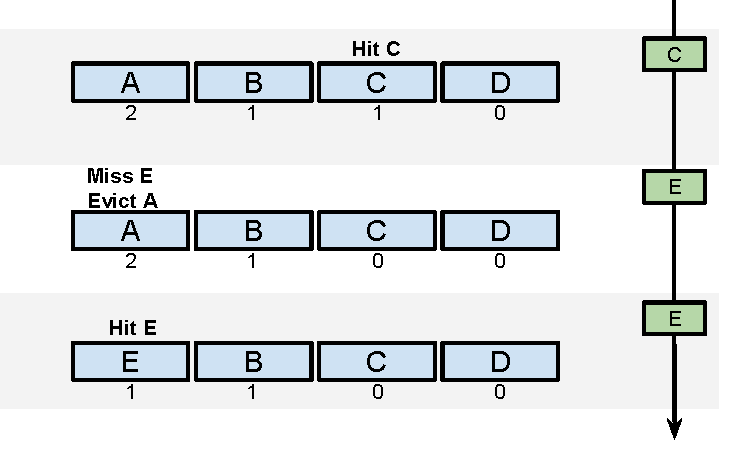
\includegraphics[width=.65\textwidth]{figures/algorithms/DRRIP}
    \caption[DRRIP managed 4-way cache set.]{DRRIP managed 4-way cache set. (M=2, static insertion)}
    \label{fig:algorithms:drrip_example}
\end{figure}

\gls{drrip}~\cite{Jaleel2010} was proposed in 2010.
\gls{drrip} does not utilize the concept of an \gls{lru} stack as done by \gls{lru} and \gls{tadip}.
In \gls{drrip}, each cache block has a number associated with it, called re-reference interval.
The re-reference interval is a relative measure of when the algorithm expects a block to be re-referenced.
Given two blocks with different re-reference intervals, then the block with a lower interval is expected to be re-referenced before the other block.
A value between 0 and $2^M - 1$ is used to represent the re-reference interval.
M is a configurable variable usually in the interval $[2, 5]$~\cite{Jaleel2010}.
The value of 0 indicates a \textit{near} re-reference interval, the algorithm expects the block to be re-referenced in the near future.
The value $2^M - 1$ indicates a \textit{distant} re-reference interval while the value of $2^M - 2$ indicates a \textit{long} re-reference interval.
Multiple blocks may have the same re-reference interval. 
Hence, blocks are not strictly ordered as in the \gls{lru} stack.
By setting $M=1$, \gls{drrip} degrades into the \gls{nru}~\cite{Microsystems2007} algorithm, which among others is used on the UltraSPARC T2.

The replacement policy of \gls{drrip} is to scan all blocks and evict the first one found with a distant re-reference interval.
If no blocks have a distant re-reference interval the re-reference interval of all blocks is incremented by one and the scan restarts.
This process repeats until the algorithm finds a victim block.
If multiple blocks are potential victims, the algorithm uses the scan order as a tie-breaker.
In the original paper, the authors specify that the leftmost potential block, the one with a lower block index, is the victim in the case of a tie.

\gls{drrip}'s promotion policy is to decrement the re-reference interval of the accessed block.
By doing this \gls{drrip} utilize access history rather than access time when calculating the re-reference interval.
Hence, to reach a near re-reference interval a block has to be accessed multiple times.
This promotion policy is different compared to \gls{lru} and \gls{tadip}, where a block will move to the \gls{mru} position following a hit, independent of the previous access history.

The insertion policy of \gls{drrip}, like \gls{dip} and \gls{tadip}, is composed of two different policies and a selection mechanism.
\gls{srrip} will always insert new blocks with a long re-reference interval. 
Depending on the state of the cache, there might be existing blocks with a higher re-reference interval than the blocks inserted by \gls{srrip}.
This gives the newly inserted blocks a chance to see a re-reference before being replaced.
\gls{brrip} is analog to \gls{bip} in \gls{dip}.
\gls{brrip} with either insert new blocks with a distant re-reference interval or, with a small probability, insert like \gls{srrip} with a long re-reference interval.
Like \gls{bip}, \gls{brrip} will allow trashing access patterns to keep some of the working set in the cache and hence improve performance over \gls{srrip}.
Selecting between the two insertion policies can be done using set dueling or \glspl{atd}, similar to what was described for \gls{tadip}.
The authors use set-dueling in their original paper, and we opt to do this in our implementation as well.

Figure~\ref{fig:algorithms:drrip_example} shows an example cache managed by \gls{drrip}.
In the example, M is set to 2, making the distant re-reference interval 3 and the long re-reference interval 2. 
Also, we assume static insertion throughout the example.
Initially, there are four blocks A, B, C and D with re-reference intervals 3, 1, 1 and 0.
First an access hits the C block, and its value decrements to 0.
Next a miss to block E occurs, block A has a re-reference interval of 3 and is evicted, E is assigned a re-reference interval of 2.
Then a miss to block D occurs, as no blocks have a re-reference interval of 3 all values are incremented by one.
After one incrementation E now has an interval of 3 and is evicted.
Then follows a hit to block D, causing its re-reference value to decrease by one.
The last row contains the final state of all blocks.